\chapter{Wprowadzenie teoretyczne}\label{chapter2}

W niniejszym rozdziale omówiono podstawowe pojęcia związane z dziedziną muzyki, syntezy dźwięku oraz przetwarzania sygnałów cyfrowych. Omówione zagadnienia odnoszą się do całości pracy, nie są one powiązane z poszczególnymi metodami syntezy. Przedstawienie ich w początkowej części pracy, ma na celu ułatwienie czytelnikowi zrozumienia kolejnych rozdziałów.



\section{Dźwięk}
Dźwięk można rozpatrywać w dwóch aspektach: fizycznym oraz muzycznym. Z fizycznego punktu widzenia, dźwięk jest zaburzeniem falowym w ośrodku sprężystym gazowym, ciekłym lub stałym, który wywołuje wrażenie słuchowe u człowieka \cite{dzwiek_pwn}. Poddziedzina fizyki, zajmująca się ściśle tematem dźwięku, nazywana jest akustyką.
% (źródło: https://encyklopedia.pwn.pl/haslo/dzwiek;3896050.html) 

W muzyce, dźwięk rozpatrywany jest jako zjawisko, które wydobywane jest z instrumentów muzycznych lub generowane za pomocą głosu ludzkiego. Główne właściwości dźwięku w muzyce, to:

\begin{itemize}
	\item wysokość dźwięku, która jest zależna od wartości częstotliwości podstawowej dźwięku (pierwszej harmonicznej),
	
	\item czas trwania - zależny od czasu emisji dźwięku na danym instrumencie,
	
	\item głośność - zależna od amplitudy drgań powietrza przenoszącego dźwięk,
	
	\item barwa dźwięku - zależna od liczby, częstotliwości poszczególnych składowych harmonicznych dźwięku oraz zmian ich amplitudy w czasie. Jako składowa harmoniczna, rozumiana jest składowa sinusoidalna dźwięku, która jest całkowitą wielkrotnością częstotliwości podstawowej danego dźwięku \cite{synth_brief_intro}.
	% (źródło: https://pl.wikipedia.org/wiki/D%C5%BAwi%C4%99k_(muzyka))
\end{itemize}

W celu ustandardyzowania dźwięków w utworach muzycznych, wprowadzono skale dźwiękowe. Obecnie w muzyce europejskiej stosowana jest skala dwunastotonowa równomiernie temperowana. Odległości między tymi dźwiękami nazywane są interwałami, które wyraża się w jednostkach półtonów. Istnieje zależność między kolejnymi półtonami. Może ona być wyrażona wzorem:
\begin{equation} \label{equ:idft}
k = f(\sqrt[12]{2})^{n}
\end{equation}
\begin{tabular}{ l l l l}
	gdzie: 	&	$f$ & - &  częstotliwość tonu dźwięku, od którego liczona jest odległość n, \\
	&	$k$ & - &  szukana częstotliwość tonu, do którego liczona jest odległość n, \\
	&   $n$ &  - & odległość tonu o częstotliwości f od tonu o częstotliwości k w półtonach, \\
\end{tabular}

Odstęp między pierwszym a ostatnim dźwiękiem w skali nazywany jest oktawą. Mierzy on 12 półtonów. Odległość ta jest wyjątkowa, gdyż dźwięk położony o oktawę dalej od pierwszego, jest jego dwukrotnością pod względem częstotliwości podstawowej składowej harmonicznej.



\section{Rodzaje klawiatur muzycznych}
Podstawowy podział klawiatur muzycznych rozpatruje się pod względem możliwości wydobycia jednego lub kilku dźwięków przy naciśnięciu kilku klawiszy. Rodzaje te nazwano klawiaturami monofonicznymi oraz polifonicznymi.

\subsection{Klawiatura monofoniczna}
Monofonia w muzyce to faktura muzyczna utworzona z pojedynczej linii melodycznej. Aby aktualnie wykonywany fragment utworu można było nazwać monofonicznym, w poszczególnych chwilach czasu powinien być grany tylko jeden dźwięk. W odniesieniu do klawiatury cyfrowej oraz analogowej, oznacza to, iż można za ich pomocą w danej chwili czasu wytwarzać tylko jeden dźwięk. Klasycznym przykładem klawiatury monofonicznej jest syntezator analogowy Minimoog.

\subsection{Klawiatura polifoniczna}
Polifonia w muzyce oznacza występowanie kilku linii melodycznych w tym samym czasie. Polifonia klawiatury zatem oznacza możliwość wydobycia w danym momencie czasu wielu dźwięków, poprzez naciśnięcie kilku klawiszy. Pojęcie polifonicznej klawiatury muzycznej nie definiuje dokładnej liczby wydobywanych się za jej pomocą dźwięków. Obecnie produkowane cyfrowe instrumenty muzyczne posiadają ograniczoną liczbę możliwych do wydobycia na raz dźwięków. Spowodowane jest to niewystarczającą mocą obliczeniową procesorów DSP.

%
% Voice allocation alghorithm - opisac jaki bedziemy uzywac
%

Jednym z głównych zadań niniejszego projektu magisterskiego jest implementacja polifonicznej klawiatury muzycznej.



\section{Przegląd metod syntezy dźwięku}
% http://legacy.spa.aalto.fi/publications/reports/sound_synth_report.pdf
Podział metod syntezy dźwięku w literaturze jest bardzo zróżnicowany. Najczęściej wykorzystuje się różnice w metodach syntezy \cite{metody_syntezy}:
\begin{itemize}
	\item metody widmowe,
	\item algorytmy abstrakcyjne,
	\item metody fizyczne,
	\item metody przetwarzania sygnału,
	% https://ieeexplore.ieee.org/document/4412805
\end{itemize}

W poniższych podrozdziałach scharakteryzowano poszczególne rodzaje metod syntezy dźwięku.

\subsection{Metody widmowe}
Do grupy widmowych metod syntezy dźwięku zaliczana jest synteza subtraktywna oraz addytywna. Zgodnie z nazwą, skupiają się one na syntezie brzmień w dziedzinie częstotliwości. Metoda subtraktywna zajmuje się głównie wycinaniem pasm widmowych z dźwieków o bogatym składzie harmonicznym. Metoda addytywna skupia się natomiast na dodawaniu kolejnych harmonicznych w dziedzinie częstotliwości. Obie metody zostały dokładnie omówione w rozdziałach \ref{chapter_subtractive} i \ref{chapter_additive} niniejszej pracy.

\subsection{Algorytmy abstrakcyjne}
% https://ccrma.stanford.edu/~bilbao/booktop/node6.html
% http://legacy.spa.aalto.fi/publications/reports/sound_synth_report.pdf
Synteza za pomocą algorytmów abstrakcyjnych zazwyczaj odnosi się do zmian istniejących już dźwięków za pomocą filtrów nieliniowych lub funkcji matematycznych. Do algorytmów abstrakcyjnych należą między innymi: synteza FM, synteza AM, synteza poprzez waveshaping lub algorytm Karplus-Strong. W literaturze można również spotkać się z określaniem tej grupy metod syntezy jako Distortion synthesis (synteza poprzez zakłócanie), która odnosi się do wprowadzanych zmian w istniejącym już dźwięku (zakłóceń). W niniejszej pracy poświęcono cały rozdział metodzie syntezy FM.

\subsection{Metody fizyczne}
% https://ccrma.stanford.edu/~bilbao/booktop/node12.html
% https://edu.pjwstk.edu.pl/wyklady/mul/scb/main37.html
Metody fizyczne skupiają się na odwzorowywaniu instrumentów muzycznych poprzez tworzenie ich modeli fizycznych. Do tej grupy należy synteza dźwięku przy użyciu modelowania matematycznego, synteza komórkowa (ang. Cellular Sound Synthesis) oraz synteza falowodowa (ang. Digital Waveguide Modeling) \cite{czyzewski_dzwiek_cyfrowy}.

Metody syntezy oparte na modelach fizycznych są uważane za najbardziej naukowe i poświęcone jest im wiele prac naukowych. W niniejszej pracy, z tej grupy metod syntezy, przedstawiono głównie syntezę fizyczną opartą o modelowanie matematyczne.

\subsection{Metody przetwarzania sygnału}
%http://marcdata.hamu.cz/vyzkum/dokumenty/Lit92.pdf - additive, subtractive, FM. sampling
%https://soundlab.cs.princeton.edu/publications/survey_icmc09.pdf - 4 strona, tabelka
%https://www.youtube.com/watch?v=I64y40EIPaM
Jako metody przetwarzania sygnału rozumiane są takie metody syntezy, które oddziaływują bezpośrednio na próbki sygnału cyfrowego. Do tej grupy metod należą między innymi: synteza tablicowa (wavetable), synteza granularna oraz synteza poprzez samplowanie.

Synteza za pośrednictwem samplowania jest najbardziej powszechną syntezą dźwięku w tej grupie metod. Polega ona na użyciu fragmentu wcześniej dokonanego nagrania (sampla) i odtwarzanie go dla różnych wysokości dźwięków. Jest to obecnie metoda najczęściej używana przez kompozytorów \cite{misra_cook_przetw_syg}.

Z uwagi na nieunaukowy charakter tego rodzaju syntezy dźwięku, żadnaej z powyższych metod nie omówiono w niniejszej pracy.



\section{Klasyczne moduły syntezatorów dźwięku}
%https://www.dummies.com/art-center/music/piano/common-keyboard-terms-and-abbreviations/
%https://en.wikipedia.org/wiki/Modular_synthesizer#:~:text=Modular%20synthesizers%20are%20synthesizers%20composed,user%20to%20create%20a%20patch.
Syntezatory analogowe nazywane są również modularnymi. Utworzenie dźwięku przez takie urządzenie wymaga przejścia sygnału przez kilka modułów. Źródłem sygnału jest zazwyczaj pewien oscylator lub generator szumu. Dźwięk jest tworzony w źródle, a następnie trafia do filtru. Następnie po filtracji jest wyprowadzany na wyjście układu.

\begin{figure}[H]
	\centering
	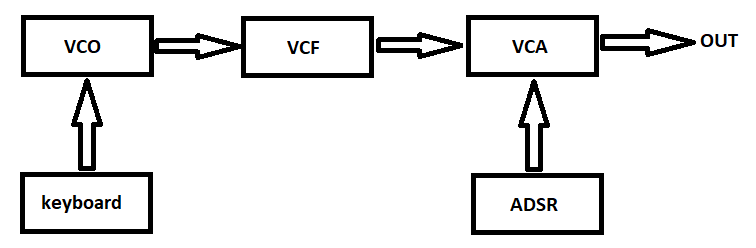
\includegraphics[width=12cm]{./grafiki/analog_synth_scheme}
	\captionsetup{justification=centering}
	\caption{Schemat podstawowego syntezatora modularnego (analogowego).}
	\label{rys:analog_scheme}
\end{figure}

Na rysunku \ref{rys:analog_scheme} przedstawiono podstawowy schemat syntezatora modularnego. Składa się on z najbardziej uniwersalnych elementów stosowanych w analogowej syntezie dźwięku. Sygnał jest tworzony przy wykorzystaniu oscylatora (VCO), którego częstotliwość zostaje ustalona poprzez naciśnięcie odpowiedniego klawisza (na klawiaturze sterującej). Następnie dźwięk, za pomocą filtru (VCF) zostaje pozbawiony pewnej części składowych harmonicznych. W dalszej kolejności dociera on do modułu sterującego amplitudą dźwięku (VCA), który ustala jego amplitudę zgodnie z ustawieniami modułu ADSR. Następnie dźwięk jest wyprowadzany na wyjście, czyli do zestawu nagłośnieniowego.

W cyfrowej syntezie dźwięku, każdy z omówionych modułów jest realizowany jako część programu komputerowego procesora klasy DSP. Poniżej opisano bardziej szczegółowo moduł, który będzie realizowany jako część programu autorskiego projektu dyplomowego.

\subsection{ADSR}
Akronim, który jest tytułem tego podrozdziału, oznacza cztero-etapowy generator obwiedni stosowany w syntezatorach. Jest on wykorzystywany zarówno w syntezatorach analogowych, jak i cyfrowych.

% źródło: D:/Data/Studia/Magisterka/Literatura%20wstepna/synthesizers__a_brief_introduction.pdf
\begin{figure}[H]
	\centering
	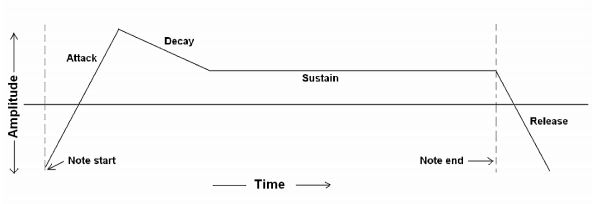
\includegraphics[width=15cm]{./grafiki/ADSR}
	\captionsetup{justification=centering}
	\caption{Generator obwiedni dźwięku (ADSR).}
	\label{rys:ADSR}
\end{figure}

Na rysunku \ref{rys:ADSR} przedstawiono przykładową obwiednie dźwięku. Poniżej wytłumaczone zostały kolejne etapy ADSR:
\begin{enumerate}
	\item Attack - czas narastania amplitudy od zera do maksimum, rozpoczyna się, gdy klawisz zostaje naciśnięty.
	
	\item Decay - czas opadania amplitudy od maksymalnej wartości do poziomu podtrzymania dźwięku.
	
	\item Sustain - poziom amplitudy przy podtrzymaniu dźwięku. Trwa dopóki klawisz nie zostanie puszczony.
	
	\item Release - czas opadania amplitudy dźwięku od poziomu wyznaczonego przez etap Sustain do wartości zero.
\end{enumerate}
Moduł ADSR może być używany niezależnie od metody syntezy dźwięku.

\section{Analogowa i cyfrowa synteza dźwięku}
Debata na temat tego, który rodzaj syntezatorów jest lepszy, trwa od samego wprowadzenia cyfrowych syntezatorów (CS) do sprzedaży. Argumenty za i przeciw obu stron tego konfliku zazwyczaj odnoszą się do charakteru brzmienia obu rodzajów syntezatorów. Nie jest to jednak jedyna właściwość syntezatorów poróżniająca obie strony.

% Porownanie: https://www.synthtopia.com/content/2019/01/11/analog-vs-digital-synthesizer-blind-test/  W opisie na YT sa wyniki
Lorenzo Furlanetto utworzył test ślepego (ang. blind test) porównania klasycznego analogowego syntezatora (AS) oraz jego cyfrowej emulacji \cite{synthtopia}. Wyniki testu pokazały, iż 51 procent ankietowanych rozpoznało, który z syntezatorów był analogowy, natomiast aż 57 procent osób orzekło, iż dźwięk syntezatorów cyfrowych jest przyjemniejszy. Oznacza to, że trudno jest odróżnić dźwięk obu typów syntezatorów, oraz że większość słuchaczy preferuje brzmienia cyfrowe.

% https://blog.andertons.co.uk/labs/hardware-synths-vs-software-synths
Syntezatory cyfrowe, w stosunku do analogowych, posiadają wiele zalet. Za pomocą tych pierwszych można dokonać syntezy wielu rodzajów dźwięków, w tym również takich, które imitują brzmienia prawdziwych instrumentów. Analogowe syntezatory natomiast, pozwalają jedynie na uzyskanie prostych brzmień, za pomocą filtracji i zmian podstawowej grupy przebiegów (trójkątnych, prostokątnych, sinusoidalnych i piłokształtnych). 
Przewaga CS uwydatnia się szczególnie w przypadku łączenia wielu instrumentów cyfrowych i jednoczesnym wykonywaniu dźwieków za pomocą jednej klawiatury \cite{andertons}.

% zrobić skróty CS (cyfrowy syntezator) i AS (analogowy syntezator)

Z technicznego punktu widzenia, CS pozwalają również na wykorzystanie w procesie generacji dźwięku cyfrowych metod przetwarzania sygnałów. Parametry na przykład filtrów cyfrowych lub innych algorytmów nie ulegają degradacji z czasem, jak również można uzyskiwać ich charakterystyki o dowolonych kształach. Natomiast elementy składowe analogowych syntezatorów należy wymieniać lub dostrajać.

% +pamięć ustawien - łatwa konfiguracja
% pamięć RAM - nowe mozliwosci generowania sygnałów
% sampling
% nowe metody syntezy

\section{MIDI}
Cyfrowy interfejs instrumentów muzycznych (MIDI) to standard utworzony w 1983 roku, służący do przekazywania informacji pomiędzy cyfrowymi instrumentami muzycznymi. Zrewolucjonizował on sektor muzyki elektronicznej. Dzięki wdrożeniu tego protokołu, muzycy mogli używać na scenie jednej klawiatury muzycznej podłączonej do wielu modułów dźwiękowych, co nie było możliwe w erze syntezatorów analogowych. MIDI zawiera zarówno standard warstwy sprzętowej, jak i zestaw komend służących do komunikacji pomiędzy urządzeniami.

\subsection{Warstwa sprzętowa MIDI}
W interfejsie MIDI, informacje przesyłane są za pomocą szeregowego połączenia dwóch urządzeń cyfrowych, w trybie półdupleks. Szybkość przesyłu informacji została ustandardyzowana i wynosi 31250 bitów na sekundę \cite{dokumentacja_midi}. 
Podobnie jak w popularnym interfejsie UART, początek transmisji ramki danych rozpoczyna bit startu o wartości 0, natomiast kończy bit stopu o wartości logicznej jedynki. Interfejs MIDI jest interfejsem prądowym, gdzie logiczne zero oznacza przepływ prądu, natomiast logiczna jedynka oznacza brak jego przepływu.

\begin{figure}[H]
	\centering
	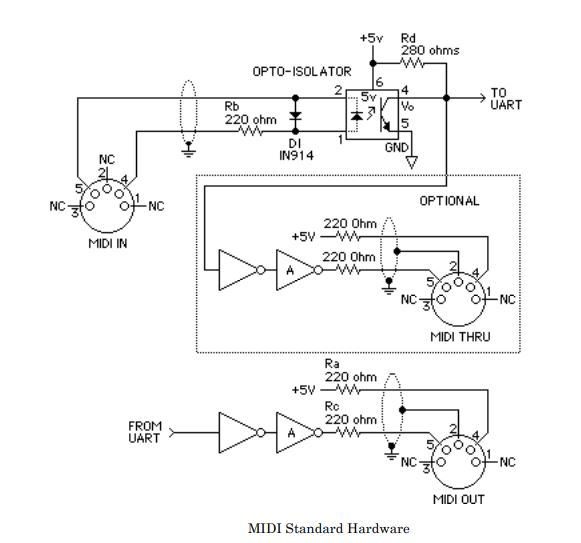
\includegraphics[width=9cm]{./grafiki/hardware_midi}
	\captionsetup{justification=centering}
	\caption{Schemat elektryczny interfejsu MIDI.}
	\label{rys:hardware_midi}
\end{figure}

Schemat sprzętowy interfejsu MIDI znajdującego się po stronie instrumentu cyfrowego przedstawiono na rysunku \ref{rys:hardware_midi}. Do połączeń z instrumentem używane są wtyki DIN pięciopinowe. Na wejściu interfejsu MIDI zawsze umieszczony zostaje transoptor, który chroni instrument otrzymujący informację przed uszkodzeniem.

\subsection{Protokół MIDI}
%https://www.midi.org/specifications-old/category/midi-1-0-detailed-specifications
%PDF: D:\Data\Studia\Magisterka\Literatura wstepna\MIDI
Wiadomości MIDI składają się z jednego bajta statusu, po którym następuje zazwyczaj jeden lub dwa bajty danych. Istnieją różne typy wiadomości MIDI. Dzieli się je na wiadomości kanałowe (odnoszące się do jednego kanału) oraz systemowe (odnoszące się do wszystkich kanałów). Wiadomości kanałowe mogą dzielić się dalej na komunikaty trybu lub komunikaty głosu. Te drugie w praktyce stanowią większość przesyłanych komunikatów w transmisji MIDI.
Komunikat głosu może nieść informację na przykład o: naciśnięciu klawisza, zwolnieniu klawisza, aftertouch (zmiana siły nacisku na klawisz, odnotowana po pewnym czasie od jego naciśnięcia), pitch bend (delikatna zmiana wysokości dźwięku). Protokół MIDI, w ramach transmisji bajta danych (komunikat głosu), może obsłużyć 128 wysokości dźwięków z jednego instrumentu. Poziom głośności, zależny od siły nacisku na klawisz, również może przyjąć jedną ze 128 wartości.

Oprócz przesyłu informacji między urządzeniami MIDI, występuje dodatkowo sygnał zegarowy MIDI (ang. MIDI Pulses), który pozwala na zsynchronizowanie kilku instrumentów, do wykonywania utworu w jednakowym tempie. Informacje zegarowe występują cyklicznie i zawsze posiadają tę samą wartość bitową.



\section{Dyskretna transformacja Fouriera}
%Technika cyfrowego przetwarzania sygnałów - A. Leśnicki
Jednym z najważniejszych narzędzi w dziedzinie cyfrowego przetwarzania sygnałów jest dyskretna transformata Fouriera (DFT). Jest to przekształcenie zdefiniowane dla skończonych sygnałów dyskretnych. Pozwala ono na transformację dyskretnego sygnału czasowego na próbki widma dyskretnego. Posiada ono również swój odpowiednik zwany IDFT, który pozwala na przekształcenie dyskretne odwrotne, z widma do sygnału czasowego \cite{lesnicki}.

\subsection{Definicja przekształcenia DFT}
%Technika cyfrowego przetwarzania sygnałów 262 strona - A. Leśnicki
Dyskretne przekształcenie Fouriera oraz odwrócone dyskretne przekształcenie Fouriera są kolejno przedstawione następującymi wzorami:
\begin{equation} \label{equ:dft}
\openup\jot
\begin{aligned}[t]
X[k] = \sum_{n=0}^{N-1} x[n]e^{-j\frac{2\pi k}{N}n} \\ 
\end{aligned}
\qquad\qquad % adjust to suit
\begin{aligned}[t]
k = 0, 1, 2, ..., N - 1 \\
\end{aligned}
\end{equation}
\begin{equation} \label{equ:idft}
\openup\jot
\begin{aligned}[t]
x[n] = \frac{1}{N}\sum_{k=0}^{N-1} X[k]e^{j\frac{2\pi n}{N}k}  \\  
\end{aligned}
\qquad\qquad % adjust to suit
\begin{aligned}[t]
 n = 0, 1, 2, ..., N - 1 \\
 \end{aligned}
\end{equation}
\begin{tabular}{ l l l l}
	gdzie: & $X[k]$ &  - & k-ta próbka widma dyskretnego sygnału, \\
	&	$x[n]$ & - &  n-ta próbka dyskretnego sygnału w dziedzinie czasu, \\
	&	$N$ & - &  liczba próbek sygnału poddanego przekształceniu Fouriera,\\
	&	$n$ & - &  próbki dyskretnego sygnału w dziedzinie czasu, \\
	&	$k$ & - &  próbki dyskretnego widma sygnału, \\
\end{tabular}

We wzorach \ref{equ:dft} i \ref{equ:idft} przyjęto indeksowanie asymetryczne. Zapis taki wybrano z uwagi na bardziej czytelną postać. W celu uproszczenia zapisu definicji DFT stosuje się współczynniki obrotu (ang. twiddle factors):
\begin{equation} \label{equ:twid_fact}
\openup\jot
\begin{aligned}[t]
	W_{N}^{kn} = e^{-j\frac{2\pi}{N}nk}  \\
\end{aligned}
\qquad\qquad % adjust to suit
\begin{aligned}[t]
   k, n = 0, 1, 2, ..., N - 1 \\
\end{aligned}
\end{equation}

Współczynniki obrotu ułatwiają obliczenia dzięki ich prostej interpretacji graficznej. Interpretowane są one jako wskazy na wykresie kołowym. Każdy ze współczynników należy rozumieć jako liczbę $e^{-j\frac{2\pi}{N}nk}$ podniesioną do potęgi $k$ razy $n$. W celu uzyskania uproszczonego zapisu definicji należy również zapisać próbki widma i sygnału w postaci wektorowej:

\begin{equation} \label{equ:dft_wekt}
\openup\jot
\begin{aligned}[t]
\mathbf{X} = 
\begin{bmatrix} 
X[0] \\ X[1] \\ ... \\ X[N-1]
\end{bmatrix}
\end{aligned}
\qquad\qquad % adjust to suit
\begin{aligned}[t]
\mathbf{x} =  
\begin{bmatrix} 
x[0] \\ x[1] \\ ... \\ x[N-1]
\end{bmatrix}
\end{aligned}
\end{equation}

Ze wzorów \ref{equ:twid_fact} i \ref{equ:dft_wekt} uzyskuje się uproszczony zapis definicji DFT:
\begin{equation} \label{equ:dft_upr}
	\mathbf{X} = [W_{N}^{kn}]\mathbf{x}
\end{equation}
\begin{equation} \label{equ:idft_upr}
\mathbf{X} = \frac{1}{N}[W_{N}^{-kn}]\mathbf{x}
\end{equation}

\subsection{Właściwości przekształcenia DFT}
%Technika cyfrowego przetwarzania sygnałów 269 strona - A. Leśnicki
Transformata DFT posiada wiele właściwości, których zastosowanie ułatwia realizację przetwarzania sygnałów cyfrowych. W poniższej tabeli przedstawiono te, które wykorzystane zostały w niniejszej pracy.

\begin{table}[H]
	\caption{Wybrane właściwości przekształcenia DFT.}
	\centering
	\label{tab:dft_wlasc}
	\begin{tabular}{|c|c|c|}
		\hline 
		\textbf{Nazwa właściwości} & \textbf{sygnał z okresem N} & \textbf{widmo DFT z okresem N} 	\\
		\hline
		Okresowość					& $x[n] = x[n + N]$ 				& $X[k] = X[k + N]$ 				\\	\hline
		Superpozycja			& $a_{1}x_{1}[n] + a_{2}x_{2}[n]$			& $a_{1}X_{1}[k] + a_{2}X_{2}[k]$			\\	\hline
		Przesunięcie cykliczne w czasie			& $x[n-K]$			& $ W_{N}^{kK}X[k]$			\\	\hline
		Korelacja cykliczna (splot kołowy)		 				& $x[n]*y^{*}[n]$			& $X[k]Y^{*}[k]$			\\ 	\hline
	\end{tabular}
\end{table}
W środkowej kolumnie tabeli \ref{tab:dft_wlasc} przedstawiono sygnał w dziedzinie czasu, a w prawej kolumnie przedstawiono odpowiednik tego sygnału w dziedzinie czestotliwości dla różnych operacji matematycznych stosowanych często w dziedzinie cyfrowego przetwarzania sygnałów.

\subsection{Algorytm FFT}
%Technika cyfrowego przetwarzania sygnałów 292 strona - A. Leśnicki
Wyznaczenie widma dyskretnego bezpośrednio z definicji \ref{equ:dft} jest bardzo złożone obliczeniowo. Przy założeniu, że próbki sygnału poddanego przekształceniu są liczbami zespolonymi, do obliczenia DFT wymagane jest $N^{2}$ mnożeń zespolonych oraz $N(N-1)$ dodawań zespolonych.

W praktyce obliczenia DFT sygnału wykonuje się z wykorzystaniem bardzo efektywnego algorytmu szybkiej transformacji Fouriera (FFT, ang. Fast Fourier Transform). Algorytm został przedstawiony w 1965 roku przez Cooleya-Tukeya i zapoczątkował nowy rozdział w dziedzinie cyfrowego przetwarzania sygnałów. Algorytm FFT można stosować również do obliczenia transformacji odwrotnej IDFT.

%https://en.wikipedia.org/wiki/File:DIT-FFT-butterfly.png
%https://pl.qwe.wiki/wiki/Butterfly_diagram
\begin{figure}[H]
	\centering
	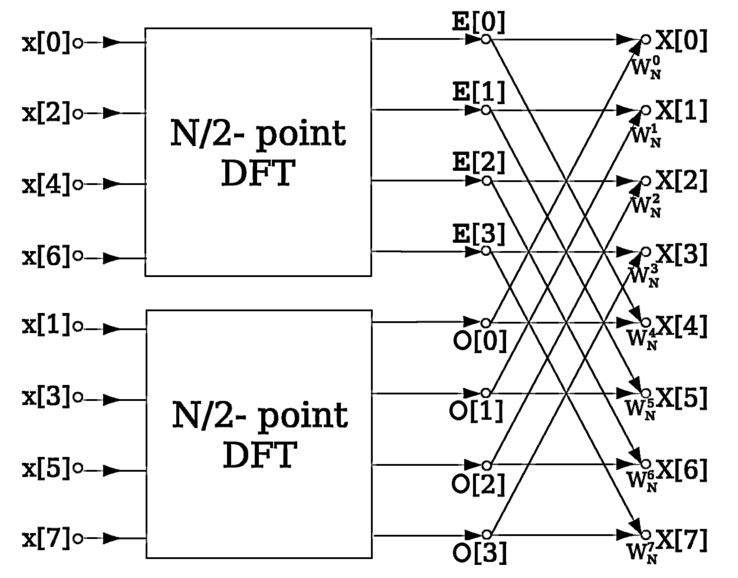
\includegraphics[width=8cm]{./grafiki/fft_motylki}
	\captionsetup{justification=centering}
	\caption{Algorytm FFT - schemat motylkowy.}
	\label{rys:fft_motyl}
\end{figure}

Algorytm FFT bazuje na metodzie dziel i zwyciężaj, dzieląc N-punktową transformację DFT na mniejsze transformacje N/2-punktowe, a następnie dokonując transformacji wyników poprzednich transformacji. Najbardziej popularną wersją algorytmu FFT jest FFT o podstawie 2, który wymaga $2^{k}$ próbek, gdzie k to liczba naturalna. Działanie algorytmu FFT o podstawie 2 opiera się na strukturach motylkowych i zostało przedstawione na rysunku \ref{rys:fft_motyl}.

%http://home.agh.edu.pl/~kkowal/DSP/FFT_wyklad.pdf
Dla liczby próbek $N$ równej $2^{k}$, występuje $log_{2}N$ poziomów algorytmu, a na każdym z nich jest $N/2$ operacji motylkowych. Ostatecznie złożoność obliczeniowa algorytmu FFT wynosi $\frac{N}{2}log_{2}N$. Pokazuje to, iż algorytm Cooleya-Tukeya jest zdecydowanie bardziej wydajny od obliczania DFT sygnału na podstawie definicji \ref{equ:dft}.
